\section{Empty lattice - 1D}
Suppose we take a very trivial example: take $V(x) = 0$, then the Schrödinger equation is very simple to solve. $V(x) = 0$ means we have free electrons.
\begin{align}
    &V(x+a) = V(x) = 0\\
    &-\frac{\hbar^2}{2m}\frac{d^2}{dx^2}\psi_k(x) = E(k)\psi_k(x)\\
    &\psi_k(x) = \frac{1}{\sqrt{L}}e^{ikx} \qquad E(k) = \frac{\hbar^2k^2}{2m} & \text{for }\frac{-G}{2} \leq k \leq \frac{G}{2} \label{eqn:solution}
\end{align}

Equation \ref{eqn:solution} gives the wave functions of the Schrödinger equation, the corresponding energies are solutions of the Schrödinger equation, too. Seen in figure \ref{fig:displacedenergybands}, when we shift our wavefunction and energy with G, we get a periodic energy spectrum. If we plot these extra potentials, we get what we call energy bands on the intersections. For a free particle, this is silly because these bandgaps have $0$ width, yet they are labeled with a gray dot.

\begin{figure}[h]
    \centering
    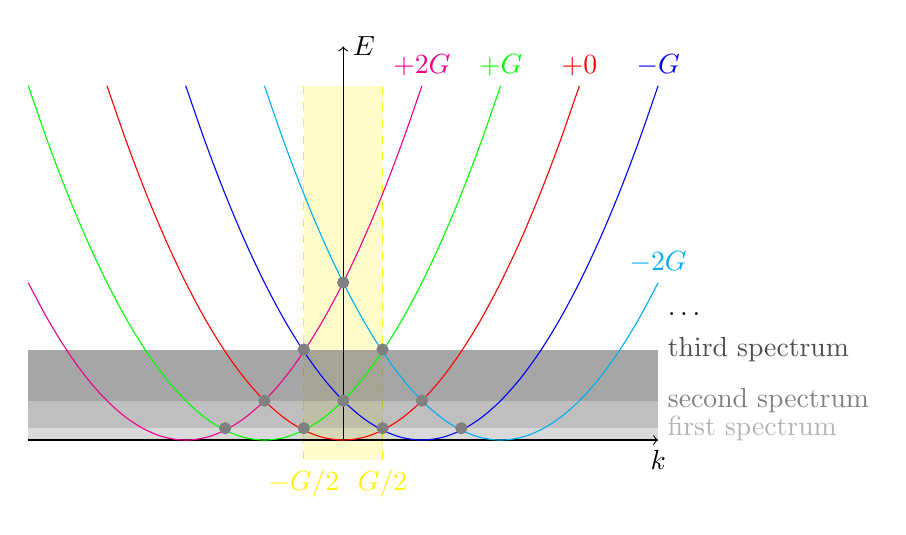
\begin{tikzpicture}
    	\draw[dashed, yellow]	(0.5, 4.5) to (0.5, -0.25) node[below]{$G/2$};
		\draw[dashed, yellow]	(-0.5, 4.5) to (-0.5, -0.25) node[below]{$-G/2$};

		\fill[fill=yellow, opacity=0.2]	(0.5, 4.5) to (0.5, -0.25) to (-0.5, -0.25) to (-0.5, 4.5);
		\fill[fill=gray, opacity=0.3]	(-4, 0.15) to (-4, 0) to (4, 0) to (4, 0.15) node[right]{first spectrum};
		\fill[fill=gray, opacity=0.5]	(-4, 0.15) to (-4, 0.5) to (4, 0.5) node[right]{second spectrum} to (4, 0.15);
		\fill[fill=gray, opacity=0.7]	(-4, 1.15) to (-4, 0.5) to (4, 0.5) to (4, 1.15) node[right]{third spectrum};

		\draw (4, 1.6) node[right]{\dots};

        \draw[->, black] (0, 0) to (0, 5) node[right]{$E$};
        \draw[->, black] (-4, 0) to (4, 0) node[below]{$k$};

		\draw[domain=-3:3, smooth, variable=\x, red] plot ({\x}, {\x*\x/2}) node[above]{$+0$};
		\draw[domain=-4:2, smooth, variable=\x, green] plot ({\x}, {(\x +1)*(\x +1)/2}) node[above]{$+G$};
		\draw[domain=-4:1, smooth, variable=\x, magenta] plot ({\x}, {(\x +2)*(\x +2)/2}) node[above]{$+2G$};
		\draw[domain=-2:4, smooth, variable=\x, blue] plot ({\x}, {(\x -1)*(\x -1)/2}) node[above]{$-G$};
		\draw[domain=-1:4, smooth, variable=\x, cyan] plot ({\x}, {(\x -2)*(\x -2)/2}) node[above]{$-2G$};

		\filldraw[gray]	(-0.5, 0.15) circle (2pt)
						(-1.5, 0.15) circle (2pt)
						(0.5, 0.15) circle (2pt)
						(1.5, 0.15) circle (2pt)
						(-1, 0.5) circle (2pt)
						(0, 0.5) circle (2pt)
						(1, 0.5) circle (2pt)
						(0.5, 1.15) circle (2pt)
						(-0.5, 1.15) circle (2pt)
						(0, 2) circle (2pt);
    \end{tikzpicture}
    \caption{Displaced energy bands with different spectra}
    \label{fig:displacedenergybands}
\end{figure}
\nt{Keep in mind that: $\frac{G}{2} - \frac{-G}{2} = \frac{2\pi}{a}$.}
\section{Nearly free electron-approximation}
Now, we include a weak preiodic potential. Then the hamiltonian becomes:
\begin{equation}
    \hat{H} = \hat{H}_0 + V(\vec{r})
\end{equation}
Where $\hat{H}$ is the free kinetic operator: $-\frac{\hbar^2}{2m}\nabla^2$ and $V(\vec{r})$ is the introduced weak potential.
We can solve it by using the pertrubation theory for solving this modified Schrödinger equation.
First solve Schrödinger for $H_0$, this gives:
\begin{align}
	&\hat{H}_0 \psi^{(0)}_{\vec{k}}(\vec{r}) = E^{(0)}_{\vec{k}} \psi^{(0)}_{\vec{k}}(\vec{r})\\
	&\qquad \Rightarrow \left\{
		\begin{array}{lr}
			\psi^{(0)}_{\vec{k}}(\vec{r}) = \frac{1}{\sqrt{V}}e^{i\vec{k}\cdot\vec{r}}\\
			E^{(0)}(\vec{k}) = \frac{\hbar^2k^2}{2m} \label{eqn:E0}
		\end{array}
	\right
\end{align}

\subsection{Pertrubation theory}
Solving with the weak potential goes as follows:
\begin{align}
    & E(\vec{k}) \approx E^{(0)}(\vec{k}) + E^{(1)}(\vec{k}) + E^{(2)}(\vec{k})\\
    & E^{(0)}(\vec{k}) = \text{ see equation \ref{eqn:E0}}\\
    & E^{(1)}(\vec{k}) =\quad <\vec{k}^{(0)} | V(\vec{r}) | \vec{k}^{(0)}>\quad = \int_{V}^{}\frac{1}{\sqrt{V}}e^{-i\vec{k}\cdot\vec{r}}V(\vec{r}) \frac{1}{\sqrt{V}}e^{i\vec{k}\cdot\vec{r}}V(\vec{r})\\
    & E^{(2)}(\vec{k}) = \sum_{\vec{k}' \neq \vec{k}} \frac{\abs{<\vec{k}^{(0)} | V(\vec{r}) | \vec{k}^{(0)}>}^2}{E^{(0)}(\vec{k}) - E^{(0)}(\vec{k}')} \label{eqn:E2}
\end{align}
\nt{We use \href{https://phys.libretexts.org/Bookshelves/Quantum_Mechanics/Quantum_Physics_(Ackland)/12\%3A_Scattering_in_Three_Dimensions/12.03\%3A_Box_Normalisation_and_Density_of_Final_States}{box normalisation}, thus putting the particle inside a box, then the k space is a sum instead of an integral. Then at the end making it unbox by making the length infinity again, we see that it works. Now, we have a more convienient way for deriving the same thing because be don't have dirac functoins anymore.}

So let's start calculating the first order approximation:
\begin{align}
    E^{(1)}(\vec{k}) &= \frac{1}{V}\int_{V}{}V(\vec{r})d\vec{r} = \tilde{V}(0) = \text{constant}\\
    E^{(2)}(\vec{k}) &= \text{ see equation \ref{eqn:E2}}\\
    \qquad \text{with: } <\vec{k}' | V(\vec{r}) | \vec{k}> \quad &= \frac{1}{V}\int_{V}{}e^{-i\vec{k}'\cdot\vec{r}}V(\vec{r})e^{i\vec{k}\cdot\vec{r}}\\
    & = \frac{1}{V}\int_{V}{}e^{i(\vec{k} - \vec{k}')\cdot\vec{r}}V(\vec{r})d\vec{r} = \tilde{V}(\vec{k} - \vec{k}')\delta_{\vec{k} - \vec{k}', \vec{G}} \label{eqn:four}
\end{align}

We see a fourier transform in equation \ref{eqn:four}, but as we know the potential $V(\vec{r})$ is periodic thus if $\vec{k}$ is not a lattice vector, the integral must be $0$. Now we can simplify the second step (equation \ref{eqn:E2}):
\begin{equation}
    \sum_{\vec{k}' \neq \vec{k}}\frac{\abs{\tilde{V}(\vec{k} - \vec{k}')\delta_{\vec{k} - \vec{k}', \vec{G}}}^2}{E^{(0)}(\vec{k}) - E^{(0)}(\vec{k}')}
\end{equation}

We rewrite this as \begin{equation} \sum_{\vec{G}}{}\frac{\abs{\tilde{V}(\vec{G})}^2}{E^{(0)}(\vec{k}) - E^{(0)}(\vec{k}')} \end{equation} by using $\vec{k} - \vec{k}' = \vec{G}$ (this is just a simple substitution using the Bragg condition (section \ref{sec:bragg}), the $\delta$-function is in this case 1).
Now we can write equation \ref{eqn:E0} in function of the derived values. Using the "normal" symbolic numeric values for the energies, we get:
\begin{equation}
    E(\vec{k}) \approx \frac{\hbar^2k^2}{2m} + \tilde{V}(0) + \frac{2m}{\hbar^2}\sum_{\vec{G}}^{}\frac{\abs{\tilde{V}(\vec{G})}^2}{k^2 - (\vec{k} - \vec{G})^2}
\end{equation}

As we see this gives a problem when the denominator is $0$, for $k^2 = (\vec{k} - \vec{G})^2$. This is the Bragg condition (section \ref{sec:bragg})!
Let's look more closely at that specific case: $E^{(0)}(\vec{k}) = E^{(0)}(\vec{k} - \vec{G})$:
\begin{equation}
\left\{
\begin{array}{lr}
    \psi^{(0)}_{\vec{k}, 1}(\vec{r}) = \frac{1}{\sqrt{V}}e^{i\vec{k}\cdot\vec{r}} & \text{with: }E^{(0)}(\vec{k}) = \frac{\hbar^2k^2}{2m}\\
    \psi^{(0)}_{\vec{k}, 2}(\vec{r}) = \frac{1}{\sqrt{V}}e^{i(\vec{k}-\vec{G})\cdot\vec{r}} & \text{with: } E^{(0)}(\vec{k}) = \frac{\hbar^2k^2}{2m}
\end{array}
\right
\end{equation}
As we can expect, this is true for multiple values for $k$. We have to deal with a degeneracy.
When you have a degeneracy, you have to span a new wavefunction into your Hilbert space, by using a linear combination of your other wavefunctions. This is Degenerate pertrubation theory, we will go over it in section \ref{sec:dpt}.

\subsection{Degenreate pertrubation theory} \label{sec:dpt}
\nt{Only if we have a degeneracy, $k^2 = (\vec{k} - \vec{G})^2$, we do this section!}
We want to find $\bar{\psi}(\vec{r}) = c_1\psi_{\vec{k}, 1} + c_2\psi_{\vec{k}, 2}$, we obtain this solution by by diagonlalizing the Hamiltonian in the new subspace:
\begin{equation}
    \left[
    \begin{array}{lr}
        H_{11} & H_{12}\\
        H_{21} & H_{22}
    \end{array}  \right]
    \left[
    \begin{array}{lr}
    c_1\\
    c_2
    \end{array}\right]
    =
    E\left[\begin{array}{lr}
    c_1\\
    c_2
    \end{array}\right] \label{eqn:hamiltonians}
\end{equation}
We will work out $H_{11}$, the other solutions are given below.
\begin{align}
    H_{11} &= \int_{V}^{}d\vec{r}\psi^*_{\vec{k}, 1}(\vec{r})\hat{H}\psi_{\vec{k}, 1}(\vec{r}) \\
    &= \int_{V}^{}d\vec{r}\frac{1}{\sqrt{V}}e^{-i\vec{k}\cdot\vec{r}}\left(\frac{-\hbar^2}{2m}\nabla^2\right)\frac{1}{\sqrt{V}}e^{i\vec{k}\cdot\vec{r}}\\
    &\qquad\qquad \text{where }\left(\frac{-\hbar^2}{2m}\nabla^2\right)\frac{1}{\sqrt{V}}e^{i\vec{k}\cdot\vec{r}} \text{ is the free energy of an electron: } E^{(0)}(\vec{k})\frac{1}{\sqrt{V}}e^{i\vec{k}\cdot\vec{r}}\nonumber\\
    &= \frac{1}{V} \int_{V}^{}E^{(0)}(\vec{k})d\vec{r} + \tilde{V}(0)\\
    &= E^{(0)}(\vec{k}) + \tilde{V}(0)
\end{align}
Because $\tilde{V}(0)$ is just a constant, we will set it to $0$. The other hamiltonians are:
\begin{align}
    & H_{12} = \tilde{V}(\vec{G}) \\
    & H_{21} = \tilde{V}(-\vec{G}) = \tilde{V}^*(-\vec{G}) \\
    & H_{22} = E^{(0)}(\vec{k} - \vec{G})
\end{align}
Now we solve equation \ref{eqn:hamiltonians} by means of a determinant, then we get:
\begin{align}
    &\left|\begin{array}{lr}
        H_{11} - E & H_{12}\\
        H_{21} & H_{22} - E
    \end{array}\right| = 0\\
    \Rightarrow E_{\pm}(\vec{k}) &= \frac{\hbar^2}{2m^2}\left(k^2 + (\vec{k} - \vec{G})^2\right)^2 \pm \frac{1}{2} \sqrt{ \left( \frac{\hbar^2}{2m} \right)^2 \left(k^2 - (\vec{k}-\vec{G})\right)^2 + 4\abs{\tilde{V}(\vec{G})}^2}
\end{align}
If we take $k^2 = (\vec{k} - \vec{G})^2$ we get $E_\pm(\vec{k}) = \frac{\hbar^2}{2m}k^2 \pm \abs{\tilde{V}(\vec{G})}$ and we can introduce gaps into our state (it still depends on our fourier transform $\tilde{V}$). The height of the introduced bandgab is: \begin{equation}\Delta E = E_+ - E_- = 2\abs{\tilde{V}(\vec{G})} \label{eqn:bandgapsize} \end{equation} \par
Let's look at this from a more practical standpoint. In figure \ref{fig:simpleEdiagram}, we plot $E^{(0)}(\vec{k})$ and one $E^{(0)}(\vec{k} - \vec{G})$, of course there are more curves but his figure is just for illustration.
\begin{figure}
    \centering
    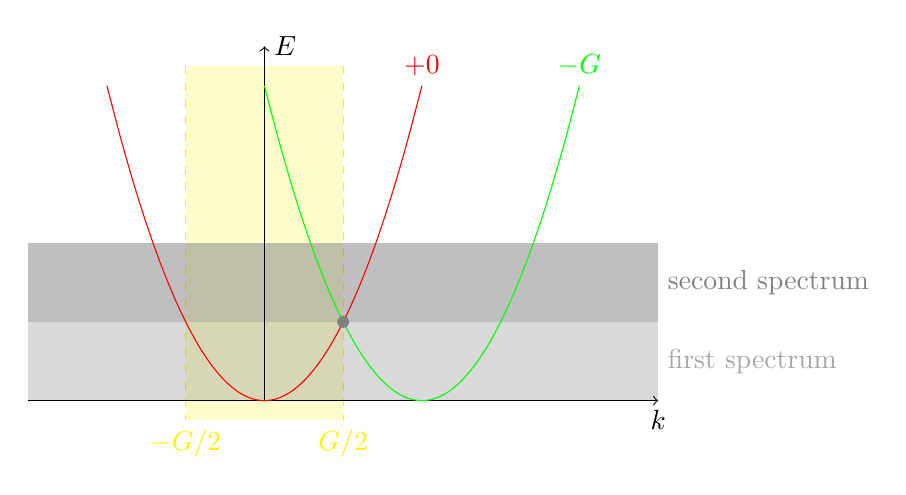
\begin{tikzpicture}
        \draw[dashed, yellow]	(1, 4.25) to (1, -0.25) node[below]{$G/2$};
		\draw[dashed, yellow]	(-1, 4.25) to (-1, -0.25) node[below]{$-G/2$};

		\fill[fill=yellow, opacity=0.2]	(1, 4.25) to (1, -0.25) to (-1, -0.25) to (-1, 4.25);
		\fill[fill=gray, opacity=0.3]	(-3, 1) to (-3, 0) to (5, 0) to (5, 1);
		\draw[gray, opacity=0.7] (5, 0.5) node[right]{first spectrum};
		\fill[fill=gray, opacity=0.5]	(-3, 1) to (-3, 2) to (5, 2) to (5, 1);
		\draw[gray] (5, 1.5) node[right]{second spectrum};
		%\fill[fill=gray, opacity=0.7]	(-3, 1.15) to (-3, 0.5) to (5, 0.5) to (5, 1.15) node[right]{third spectrum};

        \draw[->, black] (0, 0) to (0, 4.5) node[right]{$E$};
        \draw[->, black] (-3, 0) to (5, 0) node[below]{$k$};

		\draw[domain=-2:2, smooth, variable=\x, red] plot ({\x}, {\x*\x}) node[above]{$+0$};
		\draw[domain=0:4, smooth, variable=\x, green] plot ({\x}, {(\x - 2)*(\x - 2)}) node[above]{$-G$};

		\filldraw[gray]	(1, 1) circle (2pt);
    \end{tikzpicture}
    \caption{The simplified energy diagram}
    \label{fig:simpleEdiagram}
\end{figure}
\begin{figure}
    \centering
    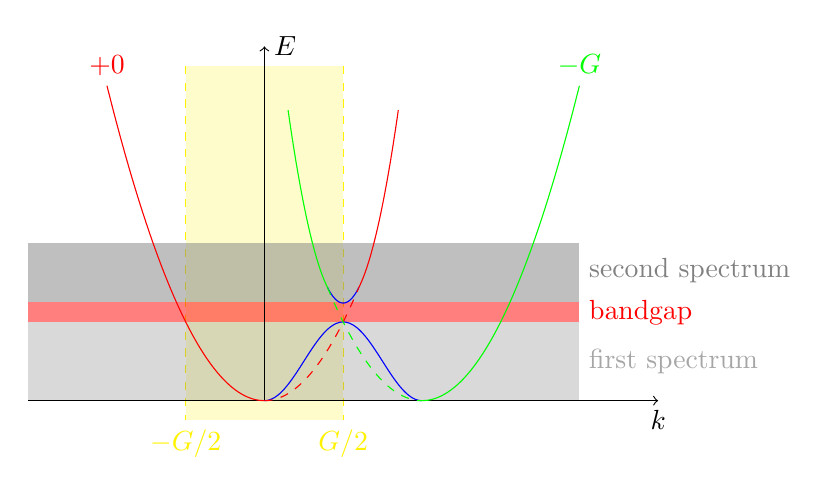
\begin{tikzpicture}
        \draw[dashed, yellow]	(1, 4.25) to (1, -0.25) node[below]{$G/2$};
		\draw[dashed, yellow]	(-1, 4.25) to (-1, -0.25) node[below]{$-G/2$};

		\fill[fill=yellow, opacity=0.2]	(1, 4.25) to (1, -0.25) to (-1, -0.25) to (-1, 4.25);
		\fill[fill=gray, opacity=0.3]	(-3, 1) to (-3, 0) to (4, 0) to (4, 1);
		\draw[gray, opacity=0.7] (4, 0.5) node[right]{first spectrum};
		\fill[fill=gray, opacity=0.5]	(-3, 1.25) to (-3, 2) to (4, 2) to (4, 1.25);
		\draw[gray] (4, 1.65) node[right]{second spectrum};
		\fill[fill=red, opacity=0.5]	(-3, 1) to (-3, 1.25) to (4, 1.25) to (4, 1);
		\draw[red] (4, 1.125) node[right]{bandgap};

        \draw[->, black] (0, 0) to (0, 4.5) node[right]{$E$};
        \draw[->, black] (-3, 0) to (5, 0) node[below]{$k$};

		\draw[domain=-2:0, smooth, variable=\x, red] plot ({\x}, {\x*\x});
		\draw[red] (-2, 4) node[above]{$+0$};
		\draw[domain=0:1, smooth, variable=\x, blue] plot ({\x}, {sin((\x - 1/2)*180)/2+1/2});
		\draw[domain=1:2, smooth, variable=\x, blue] plot ({\x}, {sin((\x - 1/2)*180)/2+1/2});
		\draw[domain=2:4, smooth, variable=\x, green] plot ({\x}, {(\x - 2)*(\x - 2)}) node[above]{$-G$};

		\draw[domain=0.3:0.8, smooth, variable=\x, green] plot ({\x}, {5*(\x - 1.2)*(\x - 0.8) + 1.44});
		\draw[domain=1.2:1.7, smooth, variable=\x, red] plot ({\x}, {5*(\x - 1.2)*(\x - 0.8) + 1.44});
		\draw[domain=0.8:1.2, smooth, variable=\x, blue] plot ({\x}, {5*(\x - 1.2)*(\x - 0.8) + 1.44});

		\draw[domain=0:1.2, dashed, smooth, variable=\x, red] plot ({\x}, {\x*\x});
		\draw[domain=0.8:2, dashed, smooth, variable=\x, green] plot ({\x}, {(\x - 2)*(\x - 2)});
    \end{tikzpicture}
    \caption{The simplified energy diagram with bandap}
    \label{fig:simpleEdiagram_withBandgap}
\end{figure}
By having degeneracies, we get a bandgab, taking the bandgap gives into consideration, we get figure \ref{fig:simpleEdiagram_withBandgap}. This bandgap is of course a forbidden zone for electrons. The size of the bandgap is given by equation \ref{eqn:bandgapsize}.\par
Now, these degeneracies can be represented in another way. As we might expect, these are repeated (or periodic) over $k$. Therefore we can stay in the first Brillouin zone (section \ref{sec:Brillouin}), this is the zone contained in $\frac{-G}{2} \leq k \leq \frac{G}{2}$, still given in yellow. This results in a structure as can be seen in figure \ref{fig:firstbrillouinzone}. Take $\frac{\pi}{a} = \frac{G}{2}$, as the Bragg point.

\begin{figure}
	\centering
	\includegraphics[scale=0.45]{./bands_in_first_brillouin_zone.jpg}
	\caption{Energy band inside the first Brillouin zone}
	\label{fig:firstbrillouinzone}
\end{figure}

\ex{1D example}{Let us use \begin{equation} V(x) = V_0\cos\frac{2\pi x}{a} \Rightarrow \tilde{V}(\pm\frac{2\pi}{a}) = \frac{V_0}{2}\end{equation} We can use this formula as it is written here because the delta functions are only defined in $\pm\frac{2\pi}{a}$ therefore we dont see the dirac functions, albeit they are there. Looking at the Bragg points:
\begin{equation} k_n = \frac{G_n}{2} = \frac{\pi}{2}n \end{equation} We can now draw the energy diagram.
\begin{center}
	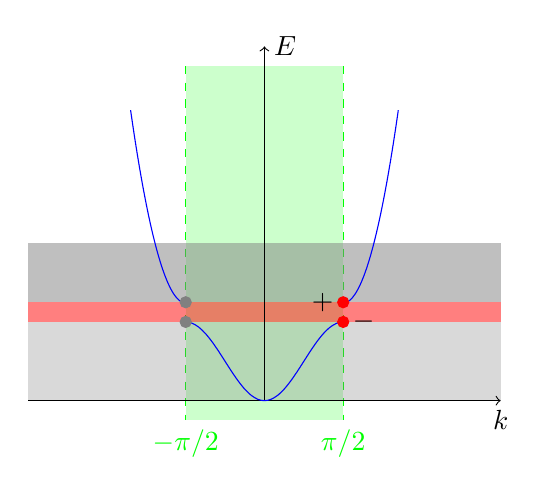
\begin{tikzpicture}
		\draw[dashed, green]	(1, 4.25) to (1, -0.25) node[below]{$\pi/2$};
		\draw[dashed, green]	(-1, 4.25) to (-1, -0.25) node[below]{$-\pi/2$};

		\fill[fill=green, opacity=0.2]	(1, 4.25) to (1, -0.25) to (-1, -0.25) to (-1, 4.25);
		\fill[fill=gray, opacity=0.3]	(-3, 1) to (-3, 0) to (3, 0) to (3, 1);
		\fill[fill=gray, opacity=0.5]	(-3, 1.25) to (-3, 2) to (3, 2) to (3, 1.25);
		\fill[fill=red, opacity=0.5]	(-3, 1) to (-3, 1.25) to (3, 1.25) to (3, 1);

		\draw[->, black] (0, 0) to (0, 4.5) node[right]{$E$};
		\draw[->, black] (-3, 0) to (3, 0) node[below]{$k$};

		\draw[domain=-1.7:-1, smooth, variable=\x, blue] plot ({\x}, {5*(\x + 1.2)*(\x + 0.8) + 1.44});
		\draw[domain=-1:1, smooth, variable=\x, blue] plot ({\x}, {sin((\x - 1/2)*180)/2+1/2});
		\draw[domain=1:1.7, smooth, variable=\x, blue] plot ({\x}, {5*(\x - 1.2)*(\x - 0.8) + 1.44});

		\filldraw[red] 	(1, 1) circle (2pt)
						(1, 1.25) circle (2pt);
		\filldraw[gray] (-1, 1.25) circle (2pt)
						(-1, 1) circle (2pt);

		\draw[black]	(1, 1) node[right]{$-$};
		\draw[black]	(1, 1.25) node[left]{$+$};
	\end{tikzpicture}
\end{center}
At the bragg points, we see a standing wave: $\psi_{\pm, k} \sim e^{i\pi x / a} \pm e^{-i\pi x/a}$, also shown in the figure in red. The bandgap is $V_0$ high.}
